\documentclass{beamer}
\mode <presentation>
{
    \usetheme{boxes}
    \usecolortheme{crane}
    \setbeamercovered{transparent}
}

\usepackage[absolute,overlay]{textpos}
\usepackage{pgf,pgfarrows,pgfnodes}
\usepackage[english]{babel}
\usepackage{lmodern}
\usepackage{newcent}
\usepackage{amsmath}
\usepackage{listings}
% math extension - one probably wants to use symbols like '[' (written as '$[$')
\usepackage{ucs}
%\usepackage[utf8]{inputenc}
%\usefonttheme{structuresmallcapsserif}

% utf8x does not work with xetex
\usepackage[utf8x]{inputenc}

\usepackage[normalem]{ulem}


\setlength{\TPHorizModule}{1mm}
\setlength{\TPVertModule}{1mm}
\newcommand{\WorkInProgress}{%
\begin{textblock}{14}(120.0,75.7)
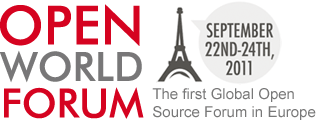
\includegraphics[height=0.1cm]{./pics/logo_owf.png}
\end{textblock}
  }

%\setbeamercolor{background canvas}{bg=\includegraphics[width=\textwidth]{./pics/wolf.png}}

\title{Assets management with~FusionInventory}
\author{\href{http://www.FusionInventory.org}{FusionInventory.org}}
\subject{Assets management with FusionInventory and GLPI}
\keywords{Assets management, Inventory, FusionInventory, GLPI}

\date{September 2011}
%\titlegraphic{GLPI}
%subtitle{\includegraphics[width=1.2cm]{./pics/fusioninventory-logo.png}}
\institute{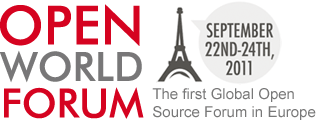
\includegraphics[height=2.2cm]{./pics/logo_owf.png}}

\titlegraphic{}
%subtitle{\includegraphics[width=1.2cm]{./pics/fusioninventory-logo.png}}
%\institute{\includegraphics[height=4.2cm]{./pics/fusioninventory-logo.pdf}}
\author{ Gonéri Le Bouder \texttt{<goneri@teclib.com>}}
\logo{\includegraphics[height=0.7cm]{./pics/fusioninventory-logo.pdf}}

\AtBeginSection[] % Do nothing for \section*
{
    \begin{frame}<beamer>
        \frametitle{Outline}
        \tableofcontents[currentsection]
    \end{frame}
}

%%%%%%%%%%%%%%%%%%%%%%%%%%%%%%%%%%%%%%%%%%%%%%%
%%%%%%%%%%%%%%%%%%%%%%%%%%%%%%%%%%%%%%%%%%%%%%%
\begin{document}

\frame[plain]{\titlepage}


\begin{frame}
    \frametitle{About us: Gonéri Le Bouder}


    \begin{block}{Free software enthusiast}
        \begin{itemize}
        \item FusionInventory project co-leader
        \item Debian Developer
        \item Perl Monger
        \item Former OCS Inventory developer
        \item Work at TECLIB', Paris, France
        \end{itemize}
    \end{block}

\end{frame}


\begin{frame}
    \frametitle{The origin}

    \begin{description}
      \item[2006] Agent creation
      \item[2008] Server project (Tracker, a GLPI plugin)
      \item[2009] Agent/Server integration 
      \item[2010] FusionInventory project
      \item[2010] Uranos integration
      \item[2011] Normation Rudder integration
      \item[2011] Mandriva Pulse2 integration (Android)
    \end{description}

\end{frame}



\begin{frame}
    \frametitle{The project infrastructure}
    %%-------------------------------------------------------------------
    %%\logo{\includegraphics[height=3.5cm]{./pics/glpi-doc.png}}
    FusionInventory is a community-driven project.

    \begin{itemize}
        \item active mailing lists
        \item IRC: \#FusionInventory on FreeNode
        \item public Forge, Git repositories, etc
    \end{itemize}
\end{frame}


\begin{frame}
    \frametitle{The FusionInventory contributors}

    \begin{center}
    \includegraphics[height=3.5cm]{./pics/sparta.jpg}
    \end{center}

    \begin{itemize}
    \item about 10 people directly involved in the project
    \item active community of contributors
    \item 2 companies involved
    \end{itemize}

    \pause
    \bf{We are looking for people to JOIN US!}
\end{frame}



\section{Global Overview}

\begin{frame}
    \frametitle{First, some vocabulary!}

    \begin{itemize}
        \item Agent: a software running one a computer
        \item Server: a software that can speak with the Agent
        \item Task: an action done by the Agent for the server 
    \end{itemize}

\end{frame}


%%
%\begin{frame}
%    \frametitle{Agent history}
%
%    \begin{center}
%    \includegraphics[height=3.5cm]{./pics/agent-smith.jpg}
%    \end{center}
%
%
%    \begin{itemize}
%        \item a fork of OCS Inventory UNIX agent by its author
%        \item started 5 years ago
%        \item GPLv2
%    \end{itemize}
%\end{frame}

%\begin{frame}
%    \begin{center}
%    \includegraphics[height=4.0cm]{pics/Perl_Foundation.pdf}
%    \end{center}
%    \frametitle{use Perl Luke!}
%
%    We choose to use Perl on the agent side.
%    \begin{itemize}
%        \item portable
%        \item reliable
%        \item versatile
%        \item stable API
%    \end{itemize}
%\end{frame}

%\begin{frame}
%    \frametitle{Agent pull}
%
%    \begin{center}
%
%%    \includegraphics[height=5.0cm]{pics/kung-fu-panda.jpg}
%
%    \end{center}
%
%\end{frame}

\begin{frame}
    \frametitle{pull / push}

    \begin{block}{FusionInventory supports "push" and "pull"}
    \begin{itemize}
    \item \textbf{"pull": Agent $\Longrightarrow$ Server} \\
    the agent creates the connection to the server.
    \item \textbf{"push": Agent $\Longleftarrow$ Server} \\
    the server awake the agent by itself.
    \end{itemize}
    \end{block}

\end{frame}

\begin{frame}
    \frametitle{Tasks}
    %
    Different Tasks are supported:
    \begin{itemize}

        \item Inventory
        \item Network discovery
        \item Remote SNMP inventory
        \item Software deployment
        \item vCenter/ESX/ESXi remote inventory
        \item Wake On Lan
    \end{itemize}
\end{frame}

\begin{frame}
    \frametitle{Servers today}

    \begin{block}{4 different servers (so far!)}
        \begin{itemize}
            \item FusionInventory for GLPI \\
            \url{http://www.FusionInventory.org}
            \item Uranos \\
            \url{http://uranos.sourceforge.net/}
            \item Rudder \\
            \url{http://www.normation.com/\#produits}
            \item OCS Inventory NG (patched to ignore the UserAgent filter) \\
            \url{http://forge.fusioninventory.org/projects/fusioninventory-agent/wiki/Patch\_ocs\_server}
        \end{itemize}
        ...local mode is also possible for Inventory
    \end{block}

\end{frame}

\begin{frame}
    \frametitle{Discution opened with}

    \begin{itemize}
    \item FusionDirectory 
    \item Mandriva's Pulse2
    \item OTRS ITSM 
    \end{itemize}
\end{frame}

%\subsection{Use cases}
%\include{purpose}


\section{Installation}

\begin{frame}
    \frametitle{Server: Installation}

    \begin{block}{FusionInventory for GLPI}
        A GLPI generic plugin.
        \begin{enumerate}
            \item Extract
            \item Configure
            \item You're done!
        \end{enumerate}
    \end{block}

\end{frame}

\begin{frame}
    \frametitle{Agent: supported OS (1/2)}

    \includegraphics[height=4.5cm]{pics/sonic.pdf}
    Runs everywhere!

    \pause

    \begin{block}{A large collection of supported OS}
        \begin{itemize}
            \item all the major system are supported
            \item portage is easy as soon as a Perl exist
        \end{itemize}
    \end{block}
\end{frame}

\begin{frame}
    \frametitle{Agent: supported OS (2/2)}
    Supported Operating Systems:

    \begin{itemize}
        \item<1-> Linux
        \item<1-> Windows, all from 2000 to Seven 64bit
        \item<1-> MacOSX 
        \item<2-> BSD
        \item<2-> AIX
        \item<2-> HP-UX
        \item<2-> Solaris
        \item<3-> Android 
    \end{itemize}


    \uncover<3->{\href{http://forge.fusioninventory.org/projects/fusioninventory-agent/wiki/Agent\_supportedplateforms}{A complete list is avallable on the website}}

\includegraphics[height=0.5cm]{pics/logos/aix.png}
\includegraphics[height=0.5cm]{pics/logos/fedora.png}
\includegraphics[height=0.5cm]{pics/logos/hp-ux.png}
\includegraphics[height=0.5cm]{pics/logos/netbsd.png}
\includegraphics[height=0.5cm]{pics/logos/openbsd.png}

\includegraphics[height=0.5cm]{pics/logos/solaris.jpg}
\includegraphics[height=0.5cm]{pics/logos/centos.jpg}

\includegraphics[height=0.5cm]{pics/logos/linux.png}
\includegraphics[height=0.5cm]{pics/logos/osx.png}
\includegraphics[height=0.5cm]{pics/logos/ubuntu.png}
\includegraphics[height=0.5cm]{pics/logos/debian.png}
\includegraphics[height=0.5cm]{pics/logos/freebsd.png}
\includegraphics[height=0.5cm]{pics/logos/redhat.png}
\includegraphics[height=0.5cm]{pics/logos/windows.jpg}
\includegraphics[height=0.5cm]{pics/logos/dragonflybsd.png}
\includegraphics[height=0.5cm]{pics/logos/mageia.png}

\end{frame}


\begin{frame}
    \frametitle{Agent: Tested systems}


 \begin{columns}
 \begin{column}[T]{4cm}
    
\includegraphics[height=4.0cm]{pics/os/linux.jpg}
 \end{column}
 \begin{column}[t]{9cm}

    \begin{block}{Linux}
        \begin{itemize}
            \item \textbf{Debian} all since 3.1
            \item \textbf{Ubuntu} all since 8.04
            \item \textbf{Mandriva} 9.2, 10.2, 2007.1, 2010.0, 2010.1
            \item \textbf{RedHat EL} (or CentOS) all since 3
            \item \textbf{Fedora} all since the 2nd
            \item \textbf{SUSE Linux Enterprise Server} 10, 11 
            \item \textbf{Slackware} 10 to 13
            \item \textbf{RedHat Linux} 7.0, 8.0 and 9.0
            \item \textbf{SME Server} 7.5
            \item \textbf{OpenSUSE} 11.3
            \item \textbf{Gentoo} 1.6.14, 2008
            \item \textbf{Montavista} 4.0 
        \end{itemize}
    \end{block}
 \end{column}
\end{columns}


\end{frame}

\begin{frame}
    \frametitle{Agent: Tested systems}

 \begin{columns}
 \begin{column}[T]{4cm}
    \includegraphics[height=4.0cm]{pics/os/windows.jpg}
 \end{column}
 \begin{column}[t]{5cm}
    \begin{block}{Windows}
        \begin{itemize}
            \item \textbf{Windows 2000} $\geq$ SP4
            \item \textbf{Windows XP} all
            \item \textbf{Windows 2003} all
            \item \textbf{Windows 2008} all
            \item \textbf{Windows Vista} all
            \item \textbf{Windows Seven} all
        \end{itemize}
    \end{block}
 \end{column}
\end{columns}

\end{frame}



\begin{frame}
    \frametitle{Agent: Tested systems}

 \begin{columns}
 \begin{column}{0.35\textwidth}
         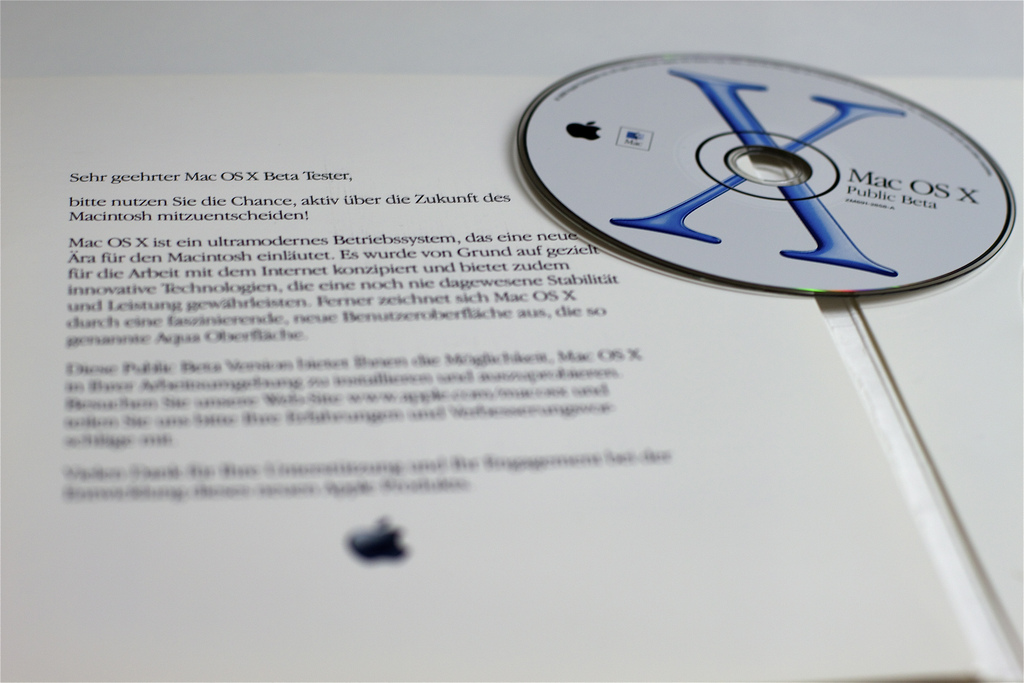
\includegraphics[height=7.5cm]{./pics/os/macosx.jpg}
 \end{column}
 \begin{column}{0.65\textwidth}
    \begin{block}{MacOSX}
        \begin{itemize}
            \item \textbf{Panther} 10.3.9 PowerPC
            \item \textbf{Tiger} all 
            \item \textbf{Leopard} all
            \item \textbf{Snow Leopard} all
        \end{itemize}
    \end{block}
 \end{column}
\end{columns}

\end{frame}

\begin{frame}
    \frametitle{Agent: Tested systems}

 \begin{columns}
 \begin{column}{0.35\textwidth}
         
\includegraphics[height=7.5cm]{./pics/os/solaris.jpg}
 \end{column}
 \begin{column}{0.65\textwidth}
    \begin{block}{Solaris}
        \begin{itemize}
            \item \textbf{Solaris} 8 to 10 for SPARC and 10 to 11 for x86
            \item \textbf{OpenSolaris} 2009.06
            \item \textbf{OpenIndiana} oi\_148
        \end{itemize}
    \end{block}
 \end{column}
\end{columns}

\end{frame}

\begin{frame}
    \frametitle{Agent: Tested systems}

\begin{columns}
 \begin{column}[T]{4cm}
    
\includegraphics[height=4.0cm]{pics/os/bsd.jpg}
 \end{column}
 \begin{column}[t]{5cm}
    \begin{block}{BSD}
        \begin{itemize}
            \item \textbf{OpenBSD} 4.5 to 4.8
            \item \textbf{FreeBSD} all since 5.3 include Debian GNU/kFreeBSD
            \item \textbf{NetBSD} 5.0 and 5.1
            \item \textbf{DragonflyBSD} 2.8
        \end{itemize}
    \end{block}
 \end{column}
\end{columns}

\end{frame}


\begin{frame}
    \frametitle{Agent: Tested systems}
\begin{columns}
 \begin{column}[T]{4cm}
%    \includegraphics[height=4.0cm]{pics/os/hpux.jpg}
 \end{column}
 \begin{column}[t]{5cm}

    \begin{block}{HPUX}
        \begin{itemize}
            \item \textbf{11.11} PA-RISC
            \item \textbf{11.23} Itanium
            \item \textbf{11.31} Itanium
        \end{itemize}
    \end{block}
 \end{column}
\end{columns}

\end{frame}

\begin{frame}
    \frametitle{Agent: Tested systems}

\begin{columns}
 \begin{column}[T]{4cm}
    \includegraphics[height=4.0cm]{pics/os/aix.jpg}
 \end{column}
 \begin{column}[t]{5cm}

    \begin{block}{AIX}
        \begin{itemize}
            \item \textbf{5.1}
            \item \textbf{5.2}
            \item \textbf{6.1}
        \end{itemize}
    \end{block}
 \end{column}
\end{columns}

\end{frame}

\begin{frame}
    \frametitle{Agent: Tested systems}

\begin{columns}
 \begin{column}[T]{4cm}
    
\includegraphics[height=4.0cm]{pics/os/android.jpg}
 \end{column}
 \begin{column}[t]{5cm}

    \begin{block}{Android}
        \begin{itemize}
            \item All revision since 1.6
            \item Available on the Market!
        \end{itemize}
    \end{block}
 \end{column}
\end{columns}
\end{frame}




\begin{frame}
    \frametitle{Agent: Installation}


    \begin{block}{different options}
        \begin{itemize}
            \item \textbf{distribution packages} \\
            \small{Debian, Fedora, EPEL, Ubuntu, Mageia, ...}
            \item \textbf{Windows installer} \\
            \small{GPO, psexec, ...}
            \item \textbf{static prebuilt packages}, untar and run \\
            \small{62 differents system so far}
            \item tarball or CPAN installation
        \end{itemize}
    \end{block}
\end{frame}




\section{Network Discovery}

\begin{frame}
    \frametitle{Network discovery}

    \begin{block}{FusionInventory can do fast network inventory using}
    \begin{itemize}
      \item NMAP 
      \item NetBios
      \item SNMP query
    \end{itemize}
    \end{block}

\end{frame}

\begin{frame}
    \frametitle{Network discovery}

    \begin{block}{During this step, we identify}
    \begin{itemize}
        \item Network information
        \item Windows domain information
        \item SNMP device name (sysdesc)
    \end{itemize}
    \end{block}
\end{frame}

\section{Remote SNMP Inventory}
%\begin{frame}
%    \frametitle{Remote SNMP inventory}
%
%    \begin{block}{Network devices}
%        \begin{itemize}
%            \item serial number, firmware, ...
%            \item ports mapping
%        \end{itemize}
%    \end{block}
%
%    \begin{block}{Network printers}
%        \begin{itemize}
%            \item serial number, firmware, ...
%            \item cartridge ink level
%            \item page counter
%        \end{itemize}
%    \end{block}
%\end{frame}


\begin{frame}
    \frametitle{SNMP: History}

%    \begin{center}
%    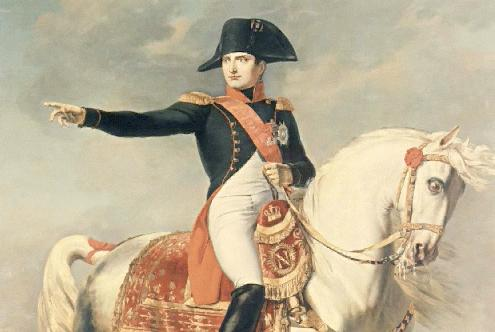
\includegraphics[height=4.0cm]{pics/napoleon.jpg}
%    \end{center}

    \begin{block}{History of SNMP}
    \begin{itemize}
    \item Standard protocole \\
    \small{First RFC: 1988}
    \item Created for monitoring devices
    \item Tree different version 1, 2c, 3 (Encryption)
    \item OID: an address per information
    \item MIB: definition of OID addresses
    \end{itemize}
    \end{block}
\end{frame}

\begin{frame}
    \frametitle{SNMP: For what?}

    \begin{block}{How we use SNMP?}
    \begin{itemize}
    \item Identify devices remotly (switch, router, printer...)
    \item Inventory devices using SNMP
    \item Get all important information
    \end{itemize}
    \end{block}
\end{frame}



\begin{frame}
    \frametitle{SNMP: The MIB nightmare?}

    \begin{block}{All people say us: MIB exist use it!}
    Yes but...
    \pause
    \begin{itemize}
    \item Most of the time hard to find
    \pause
    \item Not always free (like in FreeSoftware)
    \pause
    \item Important information may be missing
    \pause
    \item Worst! They are sometime wrong depending on device model/firmware
    \end{itemize}
    \end{block}

%    \begin{block}{With our SNMP models, we are sure device is well supported!}
%    \end{block}
\end{frame}
\begin{frame}
    \frametitle{SNMP: An example}

 \begin{columns}
 \begin{column}{0.35\textwidth}
         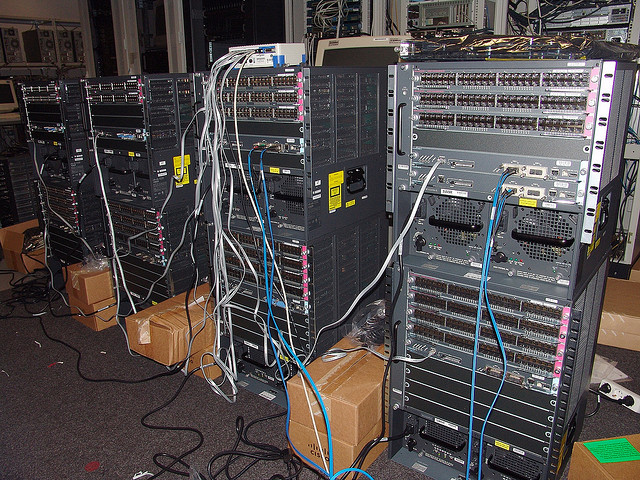
\includegraphics[height=7.5cm]{./pics/cisco.jpg}
 \end{column}
 \begin{column}{0.65\textwidth}
    \begin{block}{Example: Cisco 6500 firmware}
    12.2(33)SXI\textbf{2a} (02-Sep-09 01:00)
    \begin{itemize}
    \item Serial OID: .1.3.6.1.2.1.47.1.1.1.1.11.\textbf{1}
    \end{itemize}
    12.2(33)SXI\textbf{3} (27-Oct-09 11:12)
    \begin{itemize}
    \item Serial OID: .1.3.6.1.2.1.47.1.1.1.1.11.\textbf{2}$\Longleftarrow$ WTF?!
    \end{itemize}
    \end{block}

 \end{column}
\end{columns}


    
\end{frame}

\begin{frame}
    \frametitle{SNMP: dead teletubbies}

 \begin{columns}
 \begin{column}{0.35\textwidth}
         
\includegraphics[height=7.5cm]{./pics/dead-teletubbies.jpg}
 \end{column}
 \begin{column}{0.65\textwidth}
    \begin{block}{FAILS}
    ...
    \end{block}

 \end{column}
\end{columns}


    
\end{frame}



\begin{frame}
    \frametitle{SNMP: How do we unfuck this mess?}

    \begin{block}{We create our own MIB like files}
    \begin{itemize}
    \item XML files 
    \item Relation between OID and information \\
        \small{e.g: serial number is oid .1.3...}
    \item Simple or dynamic OID \\
        \small{a serial number or name of each port}
    \end{itemize}
    \end{block}


%    \begin{block}{How we make them?}
%    \begin{itemize}
%    \item We use a complete snmpwalk of each device + model + firmware
%    \item Our tool permit to preselect and select OID 
%    \item This tool will create and export models 
%    \end{itemize}
%    \end{block}
\end{frame}

\begin{frame}
    \frametitle{SNMP: Network switch (1/3)}

    \begin{block}{Network switch}
    \begin{itemize}
    \item Serial number
    \item Manufacturer
    \item Model
    \item Firmware
    \item Mac address    
    \item CPU/RAM load
    \item etc
    \end{itemize}
    \end{block}
\end{frame}

\begin{frame}
    \frametitle{SNMP: Network switch (2/3)}

    \begin{block}{Switch port}
    \begin{itemize}
    \item Name
    \item Network speed
    \item Port status (enabled / disabled)
    \item Errors input \& output
    \item VLAN
    \item Trunk (tagged)
    \item Active connection
    \end{itemize}
    \end{block}
\end{frame}

\begin{frame}
    \frametitle{SNMP: Network switch (3/3)}

    \begin{block}{Connections per port}
    \begin{itemize}
    \item Mac addresses \\ 
    one or many on some case
    \item LLDP and CDP neighborhood \\
        dialog and information between switches
    \end{itemize}
    \end{block}
\end{frame}

\begin{frame}
    \frametitle{SNMP: What results for switch?}

    \begin{center}
    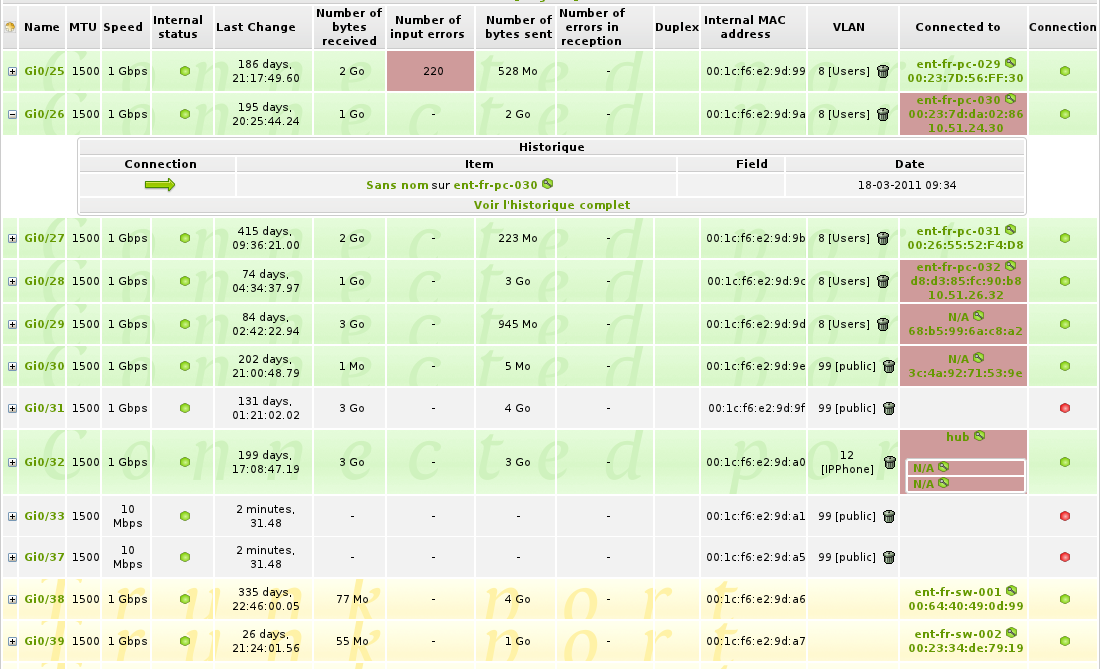
\includegraphics[width=11.7cm]{./pics/switch_ports.png}
    \end{center}
\end{frame}

\begin{frame}
    \frametitle{SNMP: Printer (1/2)}

    \begin{block}{Get printer information}
    \begin{itemize}
    \item Serial number
    \item Manufacturer
    \item Model
    \item Firmware
    \item Memory
    \item Mac address
    \item etc
    \end{itemize}
    \end{block}
\end{frame}

\begin{frame}
    \frametitle{SNMP: Printer (2/2)}

    \begin{block}{Additional important information}
    \begin{itemize}
    \item Get cartridges ink level
    \item Page counter
    \end{itemize}
    \end{block}
\end{frame}

\begin{frame}
    \frametitle{SNMP: What result for printer?}

    \begin{center}
    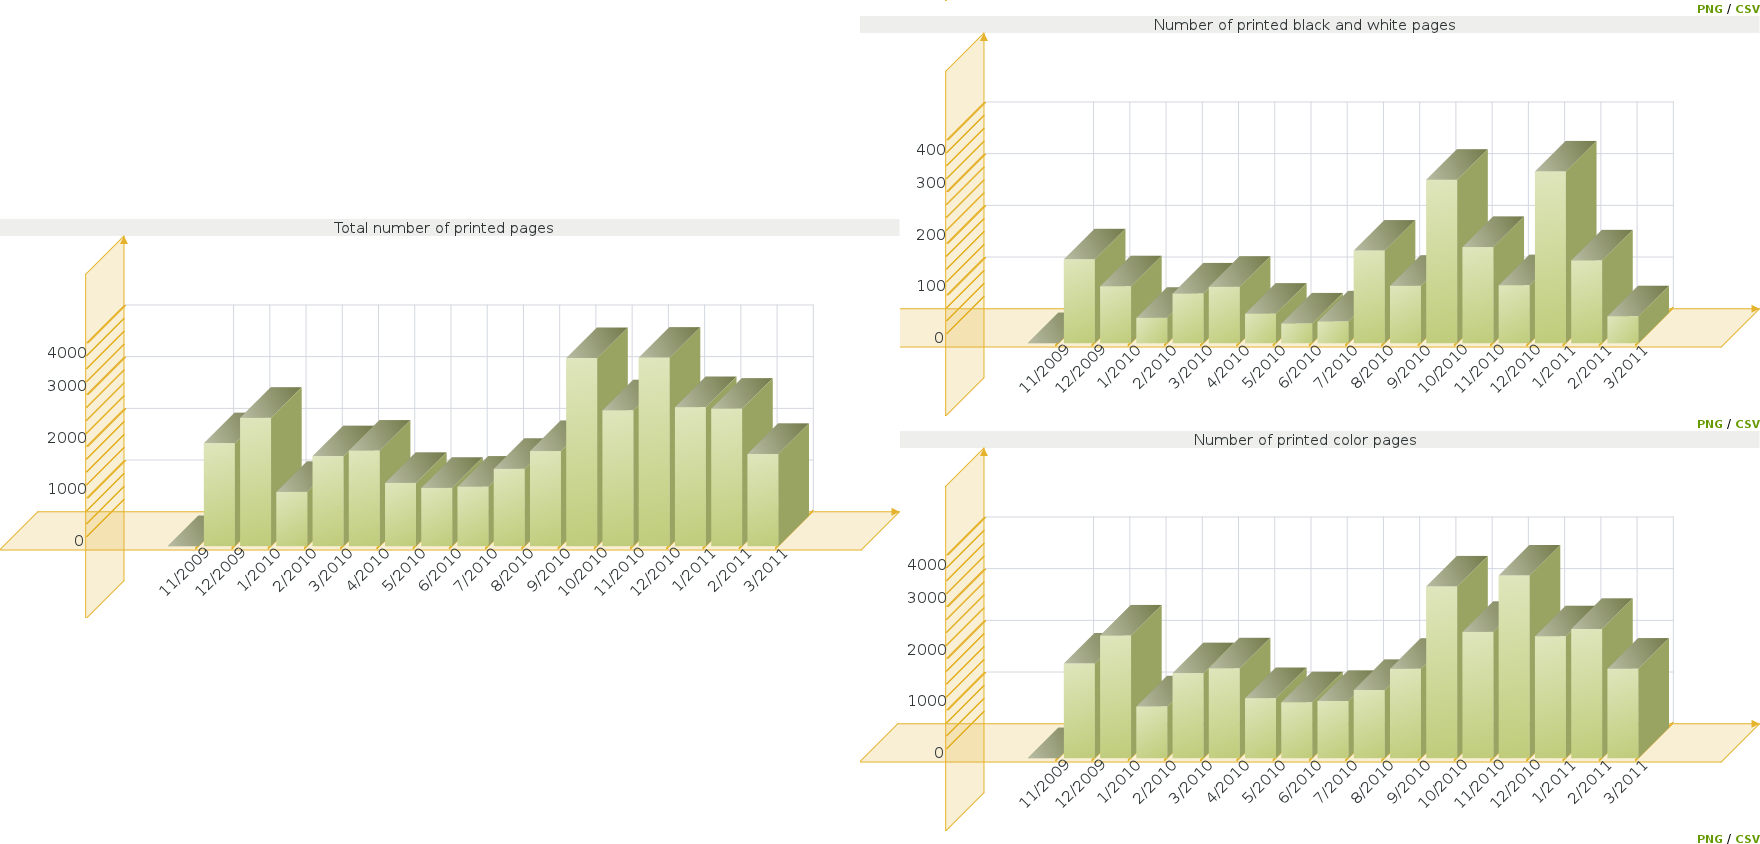
\includegraphics[width=11.7cm]{./pics/printer_graph.png}
    \end{center}
\end{frame}

\section{Wake On Lan}

\begin{frame}
    \frametitle{Wake On Lan}

    \begin{block}{What?}
    \begin{itemize}
        \item awake computer.
    \end{itemize}
    \end{block}

\pause

    \begin{block}{How?}
        Send the Magic Packet with agent
    \begin{itemize}
	\item Raw ethernet packet (only from linux computer)
	\item else, UDP packet
    \end{itemize}
    \end{block}

\pause

    \begin{block}{Benefit}
    \begin{itemize}
        \item no firewall issue
        \item nor special routage rule needed
    \end{itemize}
    \end{block}

\end{frame}

\begin{frame}
    \frametitle{Wake On Lan: Example (1/2)}

    \begin{block}{What we have}
    \begin{itemize}
    \item A remote site
    \item 50 computers all under windows
    \end{itemize}
    \end{block}


    \begin{block}{What we want}
    \begin{itemize}
    \item start all at same time, at 2:00 am for maintenance operation
    \end{itemize}
    \end{block}

\end{frame}

\begin{frame}
    \frametitle{Wake On Lan: Example (2/2)}

%    \begin{block}{Preparation (do it once)}
%    \begin{itemize}
%    \item Create a Virtual Machine on one of these computers
%    \item Install a Linux distribution on this (Debian, Fedora...)
%    \item Install a FusionInventory agent
%    \item It's ready ;)
%    \end{itemize}
%    \end{block}

    \begin{block}{Into GLPI with task management}
    \begin{itemize}
    \item Define computers to awake
    \item Schedule it at 2:00AM
    \item That's all
    \end{itemize}
    \end{block}

\end{frame}

\section{Software Deployment}

\begin{frame}
    \frametitle{Software Deployment}

    \begin{block}{What?}
    FusionInventory deployment
    \end{block}

    \begin{block}{Why a new software deployment?}
    \begin{itemize}
        \item Same user interface: GLPI
        \item Rights based on GLPI group/profile/entity
        \item Secure: HTTPS and sha512 
        \item Sexy interface using ExtJS
        \item Network efficiency: use P2P
    \end{itemize}
    \end{block}

\WorkInProgress
\end{frame}


\begin{frame}
    \frametitle{FusionInventory Deploy: package creation}

    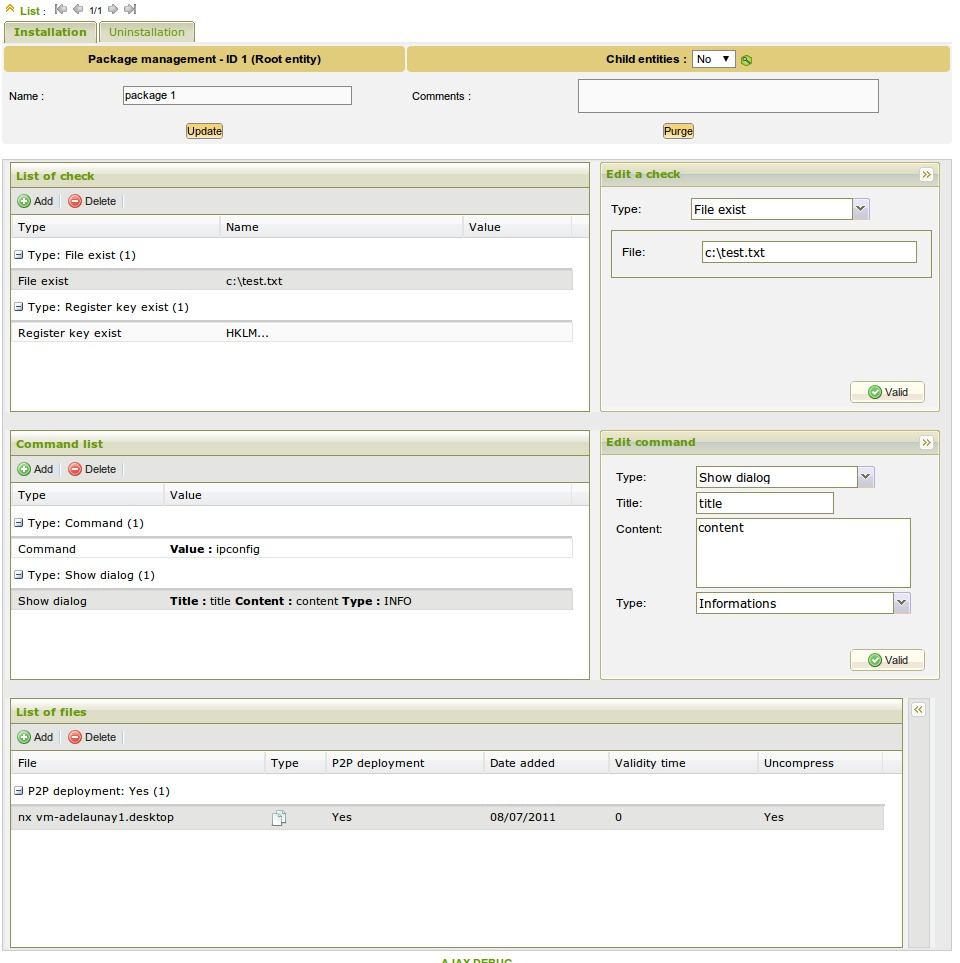
\includegraphics[height=8.0cm]{pics/packages.jpg}

\WorkInProgress
\end{frame}


\begin{frame}
    \frametitle{FusionInventory Deploy: group creation}

    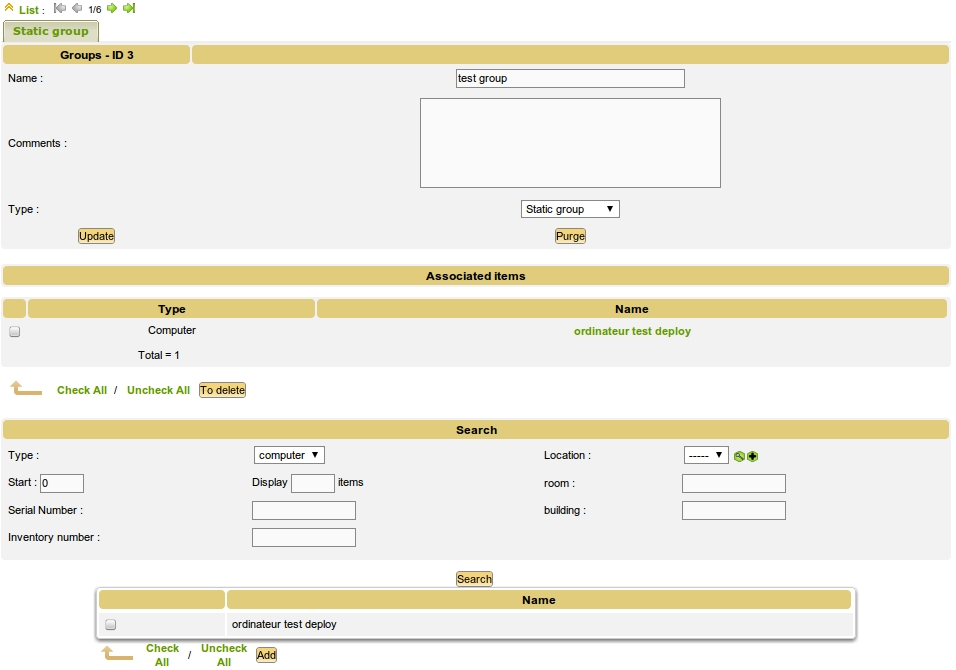
\includegraphics[height=6.0cm]{pics/groups.jpg}

\WorkInProgress
\end{frame}


\begin{frame}
    \frametitle{FusionInventory Deploy: task creation}

    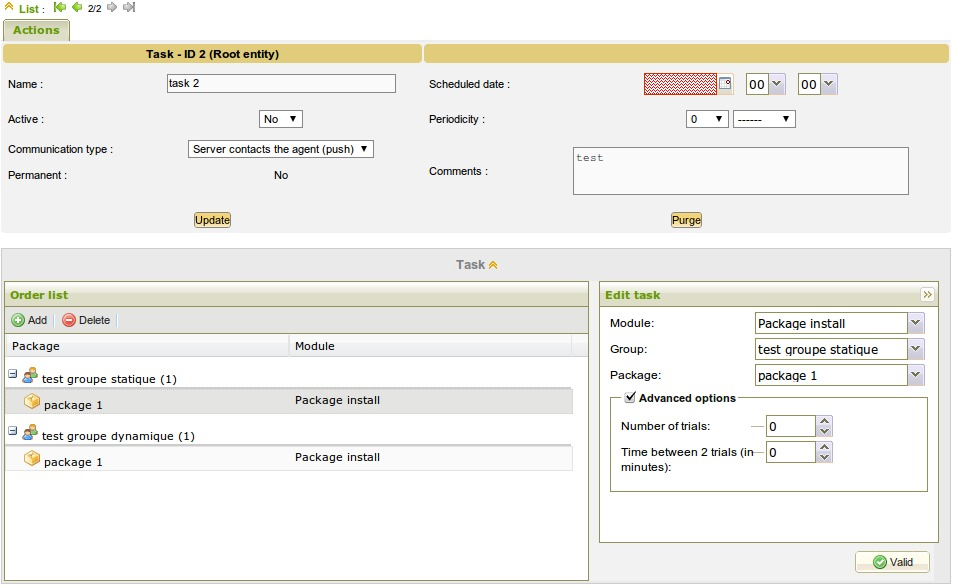
\includegraphics[height=6.0cm]{pics/tasks.jpg}

\WorkInProgress
\end{frame}

\begin{frame}
    \frametitle{FusionInventory Deploy: Work in progres}

    Release planned for the coming weeks.

    \bf{Stay turned!}

\WorkInProgress
\end{frame}


\section{vCenter/ESX/ESXi remote inventory}


\begin{frame}
    \frametitle{vCenter/ESX/ESXi}

    \begin{block}{The issue}
    You can \textbf{NOT} run an agent on these machines.
    \end{block}


\end{frame}

\begin{frame}
    \frametitle{vCenter/ESX/ESXi}

    \begin{block}{The solution}
FusionInventory is able to connect to the machine using VMware SOAP API to get:
        \begin{itemize}
                \item Hardware inventory 
                \item VirtualMachine list
        \end{itemize}
    \end{block}

    \begin{block}{vCenter}
vCenter are an interface in front of a group of ESX/ESXi.
        \begin{itemize}
                \item Hardware inventory 
                \item ESX/ESXi inventories 
        \end{itemize}
    \end{block}
\end{frame}

\begin{frame}[fragile]
    \frametitle{vCenter/ESX/ESXi: command line}

\begin{lstlisting}
fusioninventory-esx --host vcenter --user foo \ 
  --password bar --directory /tmp
\end{lstlisting}

Then you can push the generated files in the server:
\begin{lstlisting}
fusioninventory-injector -v --file /tmp/*.ocs \ 
  -u https://glpi/plugins/fusioninventory/
\end{lstlisting}

\end{frame}

\begin{frame}[fragile]
    \frametitle{vCenter/ESX/ESXi: from GLPI}

 \begin{columns}
 \begin{column}[T]{4cm}
    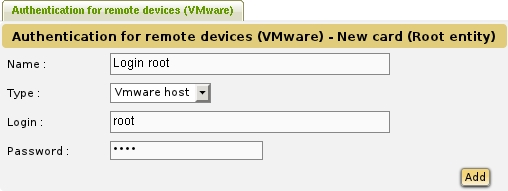
\includegraphics[height=4.0cm]{pics/esx-glpi.jpg}
 \end{column}
 \begin{column}[t]{6cm}
    \begin{block}{You can drive the ESX inventory directly from GLPI}
    \begin{itemize}
         \item Create a credential
         \item Associate it to an vCenter/ESX/ESXi server 
         \item Schedule the discovery
    \end{itemize}
    \end{block}
 \end{column}
\end{columns}




\end{frame}

\begin{frame}
\frametitle{ESX 1/2}


   \includegraphics[height=5cm]{./pics/esx1.png}
\end{frame}
%
\begin{frame}
\frametitle{ESX 2/2}


   \includegraphics[height=5cm]{./pics/esx2.png}
\end{frame}



\section{Inventory}

\begin{frame}
    \frametitle{Inventory}

    \begin{block}{The agent collects and send information}
        \begin{itemize}
            \item System: DNS, IP, AntiVirus, users, serials, etc
            \item Hardware: CPUs, storage, etc
            \item Phone configuration: SIM card, IMEI, serial
                \small{Android only}
            \item And more
        \end{itemize}
    \end{block}
\end{frame}

\section{Let's speak about Perl}

\begin{frame}
    \frametitle{Perl: Why Perl?}

    \begin{block}{A nice tool to do the job}
        \begin{itemize}
            \item A lot of data processing
            \item Some complexe data structure to deal with
            \item Few low level access
        \end{itemize}
    \end{block}
\end{frame}

\begin{frame}
    \frametitle{Perl: Portability}

    \begin{block}{A large collection of OSes supported}
        \begin{itemize}
            \item Very few difference between UNIX like OSes
            \item Win32 differences remain low
        \end{itemize}
    \end{block}
\end{frame}


\begin{frame}
    \frametitle{Perl: CPAN 1/3}

    \begin{block}{Some great pieces of software out there}
        \begin{itemize}
            \item LWP: the Perl WWW libs
            \item POE: the cooperative multitasking
            \item Win32* stuff
            \item much more
            \item Great visibility for FusionInventory distribution 
        \end{itemize}
    \end{block}
\end{frame}

\begin{frame}
    \frametitle{Perl: CPAN 2/3}

    \begin{block}{CPAN test-suite automation}
        \begin{itemize}
            \item efficiant way to get the distribution tested everywhere
        \end{itemize}
    \end{block}
\end{frame}

\begin{frame}
    \frametitle{Perl: CPAN 3/3}

    \begin{block}{Drawback}
        \begin{itemize}
            \item Some unmaintained packages
            \item XS lib are hardly portable
            \item Hard to know if a lib is thread-safe
        \end{itemize}
    \end{block}
\end{frame}



\begin{frame}
    \frametitle{Perl: System resource usage 1/3}

    \begin{block}{Memory}
        \begin{itemize}
            \item We use about 50MB on Windows
            \item fork() on Win32 is emulated and don't give back memory 
            \item No simple solution to give back memory to the OS
        \end{itemize}
        This remains lower than an AntiVirus but we plan to reduce it.
    \end{block}
\end{frame}

\begin{frame}
    \frametitle{Perl: System resource usage 2/3}

    \begin{block}{CPU}
        \begin{itemize}
            \item More expensive than C/++
        \end{itemize}
        How care if the inventory is generated in 15s instead of 5?
    \end{block}
\end{frame}

\begin{frame}
    \frametitle{Perl: System resource usage 3/3}

    \begin{block}{Disk space}
        \begin{itemize}
            \item A lot of little file → lot of I/O during install
        \end{itemize}
        A 65MB installation size is not a big deal nowaday.
    \end{block}
\end{frame}


\section{The FusionInventory::Agent distribution}

\begin{frame}
    \frametitle{Some metric (1/2)}

    \begin{block}{1,4 year ago}
        \begin{itemize}
            \item 172 Perl modules
            \item 15910 lines
            \item 0 test
        \end{itemize}
    \end{block}
\end{frame}

\begin{frame}
    \frametitle{Some metric (2/2)}

    \begin{block}{Today}
        \begin{itemize}
            \item 196 Perl modules (+11\%)
            \item 24395 lines (+15\%)
            \item 889 tests (+100\%)
        \end{itemize}
    \end{block}

\end{frame}

\begin{frame}
    \frametitle{Some metric (2/2)}

    \begin{block}{Today}
        \begin{itemize}
            \item 196 Perl modules (+11\%)
            \item 24395 lines (+15\%)
            \item \bf{889 tests (+100\%)} We enjoy boring stuff!
        \end{itemize}
    \end{block}

\end{frame}


\begin{frame}
    \frametitle{Test-Suite, aka, the boring stuff we love}

    \begin{block}{How to test untestable stuff}
        \begin{itemize}
            \item SSL certificat check for client: fire up a web server with SSL and run test
            \item various client / server protocole check
            \item ensure Win32 Modules build fine from an UNIX
            \item etc
        \end{itemize}
    \end{block}

\end{frame}

\begin{frame}
    \frametitle{What FusionInventory can bring to me?}

    \begin{block}{Different levels of integration}
        \begin{itemize}
            \item Use directly the FusionInventory Modules
            \item Call and interact with the agent
            \item Build your solution on top of GLPI using webservices 
        \end{itemize}
    \end{block}

\end{frame}

\begin{frame}
    \frametitle{What FusionInventory can bring to me?}

    \begin{block}{Improve the solution}
        \begin{itemize}
            \item Create your own "input modules" to extend inventory 
            \item Add new task 
            \item ...
        \end{itemize}
    \end{block}

\end{frame}


\section{What else?}


\begin{frame}
    \frametitle{What else? (1/2)}

    \begin{center}
    \includegraphics[height=4.0cm]{pics/whatelse.jpg}
    \end{center}

\end{frame}

\begin{frame}
    \frametitle{Our roadmap}

    What we are about to release
    \begin{itemize}
        \item FusionInventory Agent 2.2.x
        \item Software deployment
    \end{itemize}

    Work in progress
    \begin{itemize}
        \item OCS/XML → REST/JSON transition
    \end{itemize}

\end{frame}

\begin{frame}[fragile]
    \frametitle{Why JSON (1/2)}
\begin{lstlisting}
GET http://srv/?action=getConfig&machineid=foobar
{
   "httpd" : {
      "ip" : "0.0.0.0",
      "trust" : [
         "127.0.0.1" 
      ],
      "port" : 62354
   }
}
\end{lstlisting}
\end{frame}
\begin{frame}
    \frametitle{Why JSON (2/2)}


    \begin{block}{REST/JSON benefit!}
        \begin{itemize}
            \item Way simpler
            \item Already a standard in the IT management world \\
            \small{Puppet, OPSI, etc}
            \item Very small CPU/memory footprint
            \item REST is easier to debug
            \item REST is test-suite friendly using Test::HTTP::Server::Simple
        \end{itemize}
    \end{block}

\end{frame}
%
%\begin{frame}
%\frametitle{FusionInventory for GLPI 0.78: Action scheduler 1/2}
%    \includegraphics[height=7.5cm]{pics/fusion_task.pdf}
%\end{frame}
%
%\begin{frame}
%\frametitle{FusionInventory for GLPI 0.78: Action scheduler 2/2}
%    \includegraphics[height=7.5cm]{pics/walid_task_1.png}
%\end{frame}
%
%\begin{frame}
%\frametitle{FusionInventory for GLPI 0.78: Printer graph}
%    \includegraphics[height=7.5cm]{pics/walid_printer_2.png}
%\end{frame}
%%
%


%\begin{frame}
%\frametitle{OCS/XML → REST/JSON transition}
%
%\begin{block}{Why}
%    \begin{itemize}
%    \item non standard protocol
%    \begin{itemize}
%    \item unhard to extend: parameters send once whatever you do
%    \item odd XML structure to parse
%    \item hard to extend
%    \end{itemize}
%    \item more modern alternative nowaday
%    \begin{itemize}
%    \item REST
%    \item JSON
%    \end{itemize}
%    \end{itemize}
%\end{block}
%
% \begin{block}{How this will be achieved}
%    \begin{itemize}
%    \item Long transition with dual system
%    \item keep OCS inventory compatibiliy
%    \end{itemize}
%\end{block}

%\end{frame}


%
%\begin{frame}
%    \frametitle{Demo}
%
%   \includegraphics[height=5cm]{./pics/fusinvglpi.png}
%
%    \bf{Demo time!}
%\end{frame}


\section{Questions}

\begin{frame}
    \frametitle{Questions?}

%    \bf{Questions?}
    \begin{center}

    \includegraphics[height=5cm]{./pics/question.pdf}

    \end{center}
%    \includegraphics[height=7.5cm]{./pics/ask.jpg}

\end{frame}

\section{Annexe}

\begin{frame}

    \frametitle{The inventory content}

This section presents information collected in FusionInventory inventory.

\end{frame}

\begin{frame}
\frametitle{Inventory: Generic machine information (1/3)}
\begin{description}
      \item[USERID] The current user list, '/' is the delimiter. This field is deprecated, you should use the USERS section instead.
      \item[OSNAME]
      \item[OSVERSION]
      \item[OSCOMMENTS] Service Pack on Windows, kernel build date on Linux
      \item[NAME]
      \item[SWAP] The swap space in MB.
\end{description}
\end{frame}
\begin{frame}
\frametitle{Inventory: Generic machine information (2/3)}
\begin{description}

      \item[IPADDR]
      \item[WORKGROUP]
      \item[DESCRIPTION] Computer description (Windows only so far)
      \item[MEMORY] Total system memory in MB
      \item[UUID]
      \item[DNS]
      \item[LASTLOGGEDUSER] The login of the last logged user.
      \item[USERDOMAIN] This field is deprecated, you should use the USERS section instead.
      \item[DATELASTLOGGEDUSER]
\end{description}
\end{frame}
\begin{frame}
\frametitle{Inventory: Generic machine information  (3/3)}
\begin{description}
      \item[DEFAULTGATEWAY]
      \item[VMSYSTEM] The virtualization technologie used if the machine is a virtual machine.
 Can by:
 Physical: (default) Xen VirtualBox Virtual Machine: Generic if it's not possible to correctly identify the solution VMware: ESX, ESXi, server, etc QEMU SolarisZone VServer OpenVZ BSDJail Parallels Hyper-V
      \item[WINOWNER]
      \item[WINPRODID]
      \item[WINPRODKEY]
      \item[WINCOMPANY] 
      \item[WINLANG] Language code of the Windows
      \item[CHASSIS\_TYPE] The computer chassis format (e.g: Notebook, Laptop, Server, etc)
\end{description}
\end{frame}

\begin{frame}
\frametitle{Inventory: BIOS}
\begin{description}
      \item[SMODEL] System model
      \item[SMANUFACTURER] System manufacturer
      \item[SSN] System Serial number
      \item[BDATE] BIOS release date
      \item[BVERSION] The BIOS revision
      \item[BMANUFACTURER] BIOS manufacturer
      \item[MMANUFACTURER] Motherboard Manufacturer
      \item[MSN Motherboard Serial]
      \item[MMODEL] Motherboard model
      \item[ASSETTAG]
      \item[ENCLOSURESERIAL]
      \item[BASEBOARDSERIAL]
      \item[BIOSSERIAL] The optional asset tag for this machine.
\end{description}

\end{frame}
\begin{frame}

\frametitle{Inventory: PCI cards}
\begin{description}
      \item[DRIVER]
      \item[NAME] The device name, the on from the PCIIDs DB
      \item[MANUFACTURER] The manifacturer name, the on from the PCIIDs DB
      \item[PCICLASS] The PCI class ID
      \item[PCIID] The PCI ID, e.g: 8086:2a40 (only for PCI device)
      \item[PCISUBSYSTEMID] The PCI subsystem ID, e.g: 8086:2a40 (only for PCI device)
      \item[PCISLOT] The PCI slot, e.g: 00:02.1 (only for PCI device)
      \item[TYPE] The controller revision, e.g: rev 02. This field may be renamed in the future.
      \item[REV] Revision of the device in the XX format (e.g: 04)
\end{description}
\end{frame}

\begin{frame}
\frametitle{Inventory: Memories}
\begin{description}
      \item[DESCRIPTION]
      \item[FORMFACTOR] Only available on Windows, See Win32\_PhysicalMemory documentation on MSDN.
      \item[PURPOSE] Only avalaible on Windows, See Win32\_PhysicalMemory documentation on MSDN.
      \item[SPEED] In Mhz, e.g: 800
      \item[TYPE]
      \item[NUMSLOTS] Eg. 2, start at 1, not 0
      \item[SERIALNUMBER]
\end{description}
\end{frame}
\begin{frame}
\frametitle{Inventory: CPUs}
\begin{description}
      \item[CACHESIZE] The total CPU cache size in KB. e.g: 3072
      \item[CORE] Number of core.
      \item[DESCRIPTION]
      \item[MANUFACTURER] AMD/Intel/Transmeta/Cyrix/VIA
      \item[NAME] The name of the CPU, e.g: Intel(R) Core(TM)2 Duo CPU P8600 @ 2.40GHz
      \item[THREAD] Number of thread per core.
      \item[SERIAL] Serial number
      \item[SPEED] Frequency in MHz
      \item[ID] The CPU ID: \url{http://en.wikipedia.org/wiki/CPUID}
\end{description}
\end{frame}
\begin{frame}
\frametitle{Inventory: Filesystems}
\begin{description}
      \item[CREATEDATE] Date of creation of the filesystem in DD/MM/YYYY format.
      \item[DESCRIPTION]
      \item[FREE] Free space (MB)
      \item[FILESYSTEM] File system name. e.g: ext3
      \item[LABEL] Name of the partition given by the user.
      \item[LETTER] Windows driver letter. Windows only
      \item[SERIAL] Partition serial number or UUID
      \item[SYSTEMDRIVE] Boolean. Is this the system partition?
      \item[TOTAL] Total space available (MB)
      \item[TYPE] The mount point on UNIX.
      \item[VOLUMN] System name of the partition (e.g: /dev/sda1 or server:/directory for NFS)
\end{description}
\end{frame}
\begin{frame}
\frametitle{Inventory: Storage devices}
\begin{description}
      \item[DESCRIPTION] The long name of the device displayed to the user.
      \item[DISKSIZE] The disk size in MB.
      \item[INTERFACE] INTERFACE can be SCSI/HDC/IDE/USB/1394/Serial-ATA/SAS or empty if unknown
      \item[MANUFACTURER]
      \item[MODEL] The commercial name of the device
      \item[NAME] The name of the device as seen by the system.% E.g: hda (Linux), \backslash \backslash.\backslash PHYSICALDRIVE0 (Windows)
      \item[TYPE] The kind of device. There is no standard for the format of the string in this field.
      \item[SERIAL] The harddrive serial number
      \item[FIRMWARE] Firmware version
      \item[SCSI] COID, CHID, UNID and LUN
      \item[WWN] World Wide Name \url{http://fr.wikipedia.org/wiki/World\_Wide\_Name}
\end{description}

\end{frame}
\begin{frame}
\frametitle{Inventory: Softwares}
\begin{description}
      \item[NAME]
      \item[COMMENTS]
      \item[FILESIZE]
      \item[PUBLISHER]
      \item[FOLDER]
      \item[FROM] Where the information about the software came from, can be: registry, rpm, deb, etc
      \item[INSTALLDATE] Installation day in DD/MM/YYYY format. Windows only.
      \item[NO\_REMOVE] Can the software be removed.
      \item[RELEASE\_TYPE] Windows only for now, come from the registry
      \item[UNINSTALL\_STRING] Windows only, come from the registry
      \item[URL\_INFO\_ABOUT]
      \item[VERSION]
      \item[IS64BIT] If the software is in 32 or 64bit, (1/0)
      \item[GUID] Windows software GUID
\end{description}
\end{frame}
\begin{frame}
\frametitle{Inventory: Virtual machines}
\begin{description}
      \item[MEMORY] Memory size, in MB.
      \item[NAME] The name of the virtual machine.
      \item[UUID]
      \item[STATUS] The VM status: running, idle, paused, shutdown, crashed, dying, off
      \item[SUBSYSTEM] The virtualisation software. E.g: VmWare ESX
      \item[VMTYPE] The name of the virtualisation system family. The same type found is HARDWARE/VMSYSTEM
      \item[VCPU] Number of CPU affected to the virtual machine
      \item[VMID] The ID of virtual machine in the virtual managment system.
      \item[MAC The list of the MAC addresses of the virtual machine. The delimiter] is '/'. e.g: 00:23:18:91:db:8d/00:23:57:31:sb:8e
      \item[COMMENT] a comment
      \item[OWNER]
\end{description}
\end{frame}
\begin{frame}
\frametitle{Inventory: Network configuration (1/2)}
\begin{description}
      \item[A network configuration.]
      \item[DESCRIPTION] The name of the interface as seen in the OS settings, e.g: eth0 (Linux) or AMD PCNET Family Ethernet Adapter (Windows)
      \item[DRIVER] The name of the driver used by the network interface
      \item[IPADDRESS]
      \item[IPDHCP] The IP address of the DHCP server (optional).
      \item[IPGATEWAY]
      \item[IPMASK]
      \item[IPSUBNET]
\end{description}
\end{frame}

\begin{frame}
\frametitle{Inventory: Network configuration (2/2)}
\begin{description}
      \item[MACADDR]
      \item[MTU]
      \item[PCISLOT] The PCI slot name.
      \item[STATUS] Up or Down
      \item[TYPE] Interface type: Ethernet, Wifi
      \item[VIRTUALDEV] If the interface exist or not (1 or empty)
      \item[SLAVES] Bonded interfaces list in the eth0/eth1/eth2 format (/ is the separator).
      \item[MANAGEMENT] Whether or not it is a HP iLO, Sun SC, HP MP or other kind of Remote Management Interface
      \item[SPEED] Interface speed in Mb/s
      \item[BSSID] Wifi only, Access point MAC Address
      \item[SSID] Wifi only, Access point name
\end{description}
\end{frame}

\begin{frame}
\frametitle{Inventory: And also}
\begin{itemize}
      \item Logged users
      \item Battery
      \item Printer (with serial)
      \item LVM configuration (Linux, AIX $\geq$ 2.1.10)
      \item Screen and Video card
      \item USB devices
      \item Running processes
      \item Environment variables
      \item Port
      \item Slot
      \item Sound card
      \item Modem
\end{itemize}
\end{frame}




\begin{frame}
    \frametitle{Thanks}

    \begin{block}{Thanks!}
        \begin{itemize}
            \item Windows \url{http://www.flickr.com/photos/aeu04117/430338509/sizes/z/in/photostream/}
            \item AIX \url{http://www.flickr.com/photos/pchow98/5115638572/}
            \item MacOSX \url{http://www.flickr.com/photos/adriannier/5555516312/sizes/l/in/photostream/}
            \item Cisco 6500 \url{http://www.flickr.com/photos/joachim\_s\_mueller/3084164647/sizes/z/in/photostream/}
            \item Teletubbies \url{http://www.flickr.com/photos/tudor/232849285/lightbox/}
        \end{itemize}
    \end{block}
\end{frame}




\end{document}
